% Provenance (never printed): see sources/outline_sources.md (Year 3:
% Darcy's law; permeability; aquifer types; the groundwater-flow equation;
% pumping tests; solute transport, in principle).
% Brief: sources/book5/BRIEFS.md, ch. 23. Curves from figdata/bachelor-3/
% theis.py, flow_net.py and advection_dispersion.py; the site of Varden-3 from
% figdata/shared/region.py (read only). Exercise and problem values in the
% Book 5 scratch calculator calc/ch23.py. The wells, the dam, the tests and
% the solutes are invented.
\chapter{Hidrogeología}\label{ch:b3:hydrogeology}

Un pozo nuevo bombea \qty{2160}{m^3} de agua al día desde una caliza situada a unos
cientos de metros bajo una granja. Al principio nada le ocurre al pozo
propio de la granja. Un mes después su nivel de agua está casi \qty{2}{m} más bajo, aunque se encuentra
a un kilómetro de distancia y la estación de bombeo nunca ha extraído una gota de él. El
nivel del agua alrededor del pozo nuevo no ha descendido uniformemente: se ha hundido en un
cono, y este se ha extendido con rapidez a través de una roca en la que el agua
en sí misma se mueve unos pocos centímetros al día. Este capítulo construye la física que
predice ambas cifras, la rápida propagación de la presión y el lento
desplazamiento del agua, a partir de una única ley empírica hallada en 1856.
% ledger: heath:darcy

\begin{recall}
Porosidad, permeabilidad, nivel freático, agua subterránea, acuíferos, manantiales
y los pozos se han estudiado en los libros de cursos anteriores, junto con el tiempo de residencia del agua y
del agua subterránea fósil. La viscosidad, la ley de Poiseuille para el flujo en un tubo
y la ecuación de difusión se estudian en los libros de física. La función error
y las soluciones de la ecuación de difusión que la emplean se encuentran en
Capítulo~\ref{ch:b3:lithosphere-thermal-models}. Las colinas de Varden, región ficticia de la serie,
con sus areniscas, calizas, lutitas y creta, son la región de los ejercicios
desde los libros de cursos anteriores.
\end{recall}

\section{Carga hidráulica y ley de Darcy}\label{sec:b3:hydrogeology:darcy}

El agua subterránea se mueve desde donde su energía mecánica por unidad de peso es
alta hacia donde es baja. Como se mueve lentamente, su energía cinética es
despreciable, y esa energía tiene dos componentes: la altura del agua y su
presión.

\begin{definition}[Carga hidráulica; gradiente hidráulico]\label{def:b3:hydrogeology:head}
La \emph{carga hidráulica}\index{carga hidráulica} en un punto del
terreno saturado es
\[
h = z + \frac{p}{\rho g} ,
\]
la suma de la \emph{carga de elevación} $z$ del punto sobre un plano de referencia y la
\emph{carga de presión} $p/(\rho g)$, siendo $p$ la presión del agua sobre
la presión atmosférica. Es la altura a la que sube el agua en un
tubo, un piezómetro, abierto solo en ese punto. El \emph{gradiente
hidráulico}\index{gradiente hidráulico} es $\nabla h$; su módulo entre dos
puntos separados una distancia $L$ a lo largo del flujo es $\Delta h/L$.
\end{definition}

\begin{omfigure}
\centering
\begin{tikzpicture}[>=stealth, font=\small, x=1cm, y=1cm]
\fill[omLithAlluv!60] (0,-0.6) rectangle (7,3.2);
\fill[omSea!45] (0,-0.6) rectangle (7,1.9);
\draw[thick, brown!60!black] (0,3.2) -- (7,3.2);
\draw[omDef, dashed] (0,1.9) -- (7,1.9);
\node[omDef, font=\scriptsize, anchor=south east] at (6.9,1.92) {nivel freático};
% piezometer
\fill[white] (3.3,0.4) rectangle (3.7,4.0);
\draw[thick] (3.3,0.7) -- (3.3,4.0); \draw[thick] (3.7,0.7) -- (3.7,4.0);
\draw[thick, densely dotted] (3.3,0.4) -- (3.3,0.7); \draw[thick, densely dotted] (3.7,0.4) -- (3.7,0.7);
\fill[omSea!70] (3.32,0.4) rectangle (3.68,2.6);
\draw[omDef, thick] (3.3,2.6) -- (3.7,2.6);
\fill (3.5,0.55) circle (0.06);
\node[font=\scriptsize, anchor=west] at (3.75,0.55) {filtro, en el punto $P$};
% datum
\draw[black!60] (0,-0.6) -- (7,-0.6);
\node[font=\scriptsize, anchor=north west] at (0,-0.62) {plano de referencia, $z = 0$};
% heads, on the left of the tube
\draw[<->] (2.5,-0.6) -- node[left, font=\scriptsize] {$z$} (2.5,0.55);
\draw[<->] (2.5,0.55) -- node[left, font=\scriptsize] {$p/\rho g$} (2.5,2.6);
\draw[black!40, densely dashed] (2.4,0.55) -- (3.3,0.55);
\draw[black!40, densely dashed] (1.0,2.6) -- (3.3,2.6);
\draw[<->, thick, omThm] (1.1,-0.6) -- node[left, font=\scriptsize] {$h$} (1.1,2.6);
\node[font=\scriptsize, anchor=south] at (3.5,4.0) {piezómetro};
\end{tikzpicture}

\par\smallskip{\small Un piezómetro, un tubo abierto solo en su filtro. El
agua alcanza en él la \omterm{def:b3:hydrogeology:head}{carga hidráulica} del punto $P$: su carga de elevación
$z$ más su carga de presión. Aquí el nivel en el tubo está por encima del
nivel freático, como ocurre donde el agua asciende hacia un manantial o un
río.}\label{fig:b3:hydrogeology:head}
\end{omfigure}

En 1856 Henry Darcy, ingeniero francés, midió el flujo de agua a través de
columnas de arena y halló que era proporcional a la pérdida de carga por unidad de
longitud. El flujo es laminar: el agua sigue líneas de corriente separadas.
% ledger: heath:darcy

\begin{theorem}[Ley de Darcy]\label{thm:b3:hydrogeology:darcy}
En un medio poroso saturado, el volumen de agua que atraviesa la unidad de área por
unidad de tiempo es
\[
\vec q = -K\,\nabla h ,
\]
donde $K$ depende del medio y del fluido. En un medio cuyos poros
son tubos rectos paralelos de radio $a$ que ocupan una fracción $n$ del
volumen, la ley de Poiseuille proporciona esta ley con
\[
K = \frac{k\rho g}{\mu}, \qquad k = \frac{na^2}{8} ,
\]
siendo $\mu$ la viscosidad del agua.
\end{theorem}
\index{ley de Darcy}

\begin{proof}
La primera afirmación es la ley empírica de Darcy. En un tubo de radio $a$
a lo largo del flujo, la ley de Poiseuille da la velocidad media $\bar u =
-(a^2/8\mu)\,\mathrm d(p + \rho gz)/\mathrm dl = -(a^2\rho g/8\mu)\,\mathrm
dh/\mathrm dl$, puesto que $p + \rho gz = \rho g h$. Los tubos ocupan la
fracción $n$ de cualquier sección transversal, de modo que el volumen por unidad de área total es
$q = n\bar u = -(na^2/8)(\rho g/\mu)\,\mathrm dh/\mathrm dl$.
\end{proof}

Los poros reales no son tubos rectos; el teorema muestra la forma de la ley
y cómo escala. El flujo es proporcional al gradiente, al cuadrado
del tamaño de los poros, e inversamente a la viscosidad: la misma arena
deja pasar el agua más deprisa cuando está caliente.

\begin{definition}[Caudal específico; conductividad hidráulica; permeabilidad intrínseca]\label{def:b3:hydrogeology:darcy}
El \emph{caudal específico}\index{caudal específico} $\vec q$ es el
volumen de agua que atraviesa la unidad de área del medio, granos y poros
en conjunto, por unidad de tiempo. La \emph{conductividad
hidráulica}\index{conductividad hidráulica} $K$ es el coeficiente de la
\omterm{thm:b3:hydrogeology:darcy}{ley de Darcy}, en \unit{m/s} o \unit{m/d}. La \emph{permeabilidad
intrínseca}\index{permeabilidad intrínseca} del medio es $k =
K\mu/(\rho g)$, en \unit{m^2}: depende solo del medio.
\end{definition}

La \omterm{def:b3:hydrogeology:darcy}{conductividad hidráulica} de las rocas abarca doce órdenes de
magnitud, como pocas magnitudes físicas. Según el gráfico de un clásico
estudio de la materia, los intervalos típicos, en metros por día, son: arcilla
\num{e-7} a \num{e-4}; limo y loess \num{e-3} a 2; arena limosa 0.04 a
10; arena limpia 0.3 a 150; grava 100 a 4000; lutita \num{e-8} a
\num{e-4}; arenisca \num{e-5} a 0.4; rocas carbonatadas \num{e-4} cuando
solo están fracturadas, y hasta varios miles cuando son cavernosas; rocas ígneas y
metamórficas por debajo de \num{e-8} cuando no están fracturadas, y hasta unos pocos cuando
lo están. La mayoría de las rocas también conducen mejor el agua en el sentido de la estratificación que
transversalmente a ella.
% ledger: heath:darcy, heath:k-chart

El \omterm{def:b3:hydrogeology:darcy}{caudal específico} es un flujo a través de toda la sección; el agua circula
solo por los poros, y más deprisa.

\begin{definition}[Velocidad de filtración]\label{def:b3:hydrogeology:seepage}
La \emph{velocidad de filtración}\index{velocidad de filtración} es $\vec v = \vec
q/n_e$, la velocidad media del agua en los poros, siendo $n_e$ la
porosidad efectiva, la de los poros conectados a través de los que circula el
agua.
\end{definition}

Una arena gruesa con $K = \qty{60}{m/d}$, un gradiente de 1 en 1000 y una
porosidad de 0.20 mueve su agua a \qty{0.3}{m/d}; una arcilla con $K =
\qty{e-4}{m/d}$, un gradiente de 1 en 10 y una porosidad de 0.50, a
\qty{2e-5}{m/d}, menos de un centímetro al año. El agua subterránea no circula
por ríos subterráneos, salvo en las cuevas de las calizas y en los tubos de las
coladas volcánicas. Son valores medios: donde viaja un contaminante, su parte más rápida puede
ir varias veces más deprisa.
% ledger: heath:velocity

\section{Acuíferos}\label{sec:b3:hydrogeology:aquifers}

\begin{definition}[Acuíferos confinados y libres; acuitardo]\label{def:b3:hydrogeology:aquifer-types}
Un \emph{acuífero libre}\index{acuífero libre} es un acuífero cuya
superficie superior es el nivel freático. Un \emph{acuífero
confinado}\index{acuífero confinado} es un acuífero cubierto por una capa de conductividad mucho
menor, de modo que el agua que contiene está a presión: en un pozo que lo alcanza,
el agua asciende por encima del techo del acuífero hasta su superficie
piezométrica. Una capa de baja conductividad que frena, pero no detiene, el paso del agua
entre acuíferos es un
\emph{acuitardo}\index{acuitardo}.
\end{definition}

\begin{definition}[Transmisividad; coeficiente de almacenamiento; rendimiento específico]\label{def:b3:hydrogeology:storage}
La \emph{transmisividad}\index{transmisividad} de un acuífero de espesor
$b$ es $T = Kb$, el caudal por unidad de anchura con gradiente unitario, en
\unit{m^2/d}. Su \emph{coeficiente de almacenamiento}\index{coeficiente de almacenamiento}
$S$ es el volumen de agua liberado por unidad de área del
acuífero cuando la carga desciende una unidad; es adimensional. El
\emph{rendimiento específico}\index{rendimiento específico} $S_y$ de una roca es el volumen
de agua que drena por gravedad, por unidad de volumen, cuando el nivel
freático desciende a través de ella.
\end{definition}

Los dos tipos de acuífero liberan el agua de distinta manera. En un \omterm{def:b3:hydrogeology:aquifer-types}{acuífero confinado}
la carga desciende, pero los poros permanecen llenos: el agua se expande un
poco, y el acuífero, que soporta más peso de las rocas suprayacentes,
se comprime un poco. La expansión del agua por sí sola libera unos
\num{9e-7} metros cúbicos por metro cúbico de acuífero y por metro de carga;
con la compresión, el \omterm{def:b3:hydrogeology:storage}{coeficiente de almacenamiento} de la mayoría de los \omterm{def:b3:hydrogeology:aquifer-types}{acuíferos confinados} es
de \num{e-5} a \num{e-3}. En un \omterm{def:b3:hydrogeology:aquifer-types}{acuífero libre} el nivel freático desciende y
los poros situados encima drenan: el \omterm{def:b3:hydrogeology:storage}{coeficiente de almacenamiento} es el \omterm{def:b3:hydrogeology:storage}{rendimiento específico}, de unos 0.1
a 0.3, entre cien y diez mil veces mayor. Las \omterm{def:b3:hydrogeology:storage}{transmisividades} de
los acuíferos en explotación van desde menos de \qty{1}{m^2/d} en rocas fracturadas
hasta \qty{100000}{m^2/d} en calizas cavernosas y coladas de lava. Donde la
carga de un \omterm{def:b3:hydrogeology:aquifer-types}{acuífero confinado} se abate durante mucho tiempo, las arcillas que contiene
y las que lo rodean drenan y se compactan, y el terreno suprayacente se hunde.
% ledger: heath:storage, heath:transmissivity

\begin{omfigure}
\centering
\begin{tikzpicture}[>=stealth, font=\small, x=1cm, y=1.1cm]
\begin{scope}
\clip (0,-1.3) -- (0,2.0) -- (3.5,2.9) -- (5,3.5) -- (7.5,4.2) -- (11,3.8) -- (11,-1.3) -- cycle;
\fill[lith sandstone] (0,-1.3) rectangle (11,4.5);
\fill[lith limestone] (0,1.8) -- (11,-0.95) -- (11,0.05) -- (0,2.8) -- cycle;
\fill[lith shale] (0,2.8) -- (11,0.05) -- (11,1.25) -- (0,4.0) -- cycle;
\fill[omLithLime!25] (0,4.0) -- (11,1.25) -- (11,4.5) -- (0,4.5) -- cycle;
\end{scope}
\draw[thick, brown!60!black] (0,2.0) -- (3.5,2.9) -- (5,3.5) -- (7.5,4.2) -- (11,3.8);
% water table in the chalk
\draw[omDef, dashed, thick] (4.5,3.0) .. controls (6,3.35) and (8.5,3.35) .. (11,2.8);
\node[omDef, font=\scriptsize, anchor=south] at (6.6,3.32) {nivel freático};
% potentiometric surface of the limestone
\draw[omThm, densely dashdotted, thick] (1.4,2.36) -- (11,2.2);
\node[omThm, font=\scriptsize, anchor=south east, fill=white, inner sep=1pt] at (10.9,2.25) {superficie piezométrica de la caliza};
% well Varden-3
\draw[thick] (2.9,2.74) -- (2.9,1.05); \draw[thick] (3.1,2.8) -- (3.1,1.05);
\fill[omDef!35] (2.92,1.05) rectangle (3.08,2.33);
\draw[omThm, thick] (2.85,2.33) -- (3.15,2.33);
\node[font=\scriptsize, anchor=south] at (3.0,2.95) {Varden-3};
% labels
\node[font=\scriptsize, fill=white, inner sep=1pt] at (7.5,0.45) {caliza: acuífero confinado};
\node[font=\scriptsize, fill=white, inner sep=1pt] at (7.5,1.5) {lutita: capa confinante};
\node[font=\scriptsize, fill=white, inner sep=1pt] at (8.4,2.8) {creta: acuífero libre};
\node[font=\scriptsize, fill=white, inner sep=1pt] at (7.5,-0.8) {arenisca};
\node[font=\scriptsize, fill=white, inner sep=1pt, align=center] at (0.8,1.75) {caliza\\afloramiento};
\draw[->, omDef, thick] (0.8,3.0) -- (0.8,2.3);
\node[omDef, font=\scriptsize, anchor=south] at (0.8,3.0) {recarga};
\end{tikzpicture}

\par\smallskip{\small Corte esquemático de la cubierta de los montes Varden
de oeste a este, sin escala. La creta alberga un \omterm{def:b3:hydrogeology:aquifer-types}{acuífero libre}
bajo su nivel freático. La caliza jurásica se recarga donde aflora y está
confinada bajo la lutita: en el pozo Varden-3 del problema, perforado a
través de la lutita y abierto solo a la caliza, el agua asciende hasta la
superficie potenciométrica, muy por encima del techo del acuífero pero por
debajo del suelo.}\label{fig:b3:hydrogeology:aquifers}
\end{omfigure}
% ledger: region:name

\section{La ecuación del flujo de agua subterránea}\label{sec:b3:hydrogeology:flow-equation}

\begin{theorem}[Ecuación del flujo de agua subterránea]\label{thm:b3:hydrogeology:flow-equation}
En un \omterm{def:b3:hydrogeology:aquifer-types}{acuífero confinado} de \omterm{def:b3:hydrogeology:storage}{transmisividad} $T$ y \omterm{def:b3:hydrogeology:storage}{coeficiente de almacenamiento} $S$ constantes,
con flujo horizontal, la carga $h(x, y, t)$ obedece
\[
S\,\frac{\partial h}{\partial t} = T\nabla^2h + W ,
\]
siendo $W$ el volumen de agua añadido por unidad de área y de tiempo por la recarga o
extraído por bombeo (negativo). En flujo estacionario sin fuentes, $\nabla^2h =
0$.
\end{theorem}
\index{ecuación del flujo de agua subterránea}

\begin{proof}
Considérese una columna del acuífero de área $\mathrm dx\,\mathrm dy$. El caudal por
unidad de anchura a través de todo su espesor es $-T\nabla h$, por la \omterm{thm:b3:hydrogeology:darcy}{ley de
Darcy} multiplicada por $b$. El flujo neto entrante es $-\nabla\cdot(-T\nabla h)\,\mathrm dx\,\mathrm
dy = T\nabla^2h\,\mathrm dx\,\mathrm dy$. El agua almacenada en la columna
cambia a razón de $S\,(\partial h/\partial t)\,\mathrm dx\,\mathrm dy$,
por la definición de $S$. La conservación de la masa, tratando la densidad del agua
como constante en el balance, iguala el almacenamiento a la entrada más las fuentes.
\end{proof}

Es la ecuación de difusión de los libros de física, con la difusividad
hidráulica $T/S$ en lugar de una térmica. Para una caliza confinada con
$T = \qty{450}{m^2/d}$ y $S = \num{2e-4}$, la difusividad es
\qty{2.25e6}{m^2/d}: un cambio de carga se extiende a lo largo de \qty{1}{km} en
unos $L^2S/T$, medio día. La misma caliza, libre, con $S =
0.2$, tardaría mil veces más. La presión se propaga rápido, el
agua se mueve despacio: los dos números del inicio.

\begin{proposition}[Flujo radial estacionario hacia un pozo]\label{prop:b3:hydrogeology:thiem}
Un pozo bombea $Q$ desde un \omterm{def:b3:hydrogeology:aquifer-types}{acuífero confinado} de \omterm{def:b3:hydrogeology:storage}{transmisividad} $T$, siendo el flujo
estacionario y radial. Entre dos distancias $r_1 < r_2$ del pozo, los
descensos difieren en
\[
s_1 - s_2 = \frac{Q}{2\pi T}\ln\frac{r_2}{r_1} .
\]
\end{proposition}

\begin{proof}
A través de cada círculo de radio $r$ alrededor del pozo, la entrada es $Q = 2\pi r
T\,\mathrm dh/\mathrm dr$. Integrando $\mathrm dh = (Q/2\pi T)\,\mathrm
dr/r$ desde $r_1$ hasta $r_2$, y escribiendo $s = h_0 - h$, se obtiene el resultado.
\end{proof}

En dos dimensiones, el flujo estacionario se dibuja con una \omterm{def:b3:hydrogeology:flow-net}{red de flujo}.

\begin{definition}[Red de flujo]\label{def:b3:hydrogeology:flow-net}
Una \emph{red de flujo}\index{red de flujo} es un dibujo del flujo estacionario de agua subterránea en
una sección homogénea e isótropa mediante dos familias de curvas: las equipotenciales,
líneas de igual carga, y las líneas de corriente, que sigue el agua. Las
líneas de corriente cortan a las equipotenciales en ángulo recto, y en una red de flujo
se espacian de modo que las celdas son cuadrados curvilíneos.
\end{definition}

\begin{method}[Filtración a partir de una red de flujo]\label{met:b3:hydrogeology:flow-net}
\leavevmode
\begin{enumerate}
\item Dibújense los contornos: un contorno impermeable es una línea de corriente; el lecho de
  un cuerpo de agua, donde la carga es fija, es una equipotencial.
\item Dibújense $N_d$ caídas de carga entre la carga más alta y la más baja, $\Delta h
  = H/N_d$, y las líneas de corriente que forman $N_f$ canales de flujo, por tanteo,
  hasta que cada celda sea un cuadrado curvilíneo.
\item Cada canal transporta $K\Delta h$ por unidad de longitud normal a la
  sección, cancelándose la longitud y la anchura del cuadrado: el total es $q =
  KHN_f/N_d$.
\end{enumerate}
\end{method}

\begin{omfigure}
\centering
\begin{tikzpicture}
\begin{axis}[width=0.95\linewidth, height=0.36\linewidth, axis equal image,
  xmin=-60, xmax=60, ymin=-20, ymax=13, xlabel={$x$ (\unit{m})}, ylabel={$z$ (\unit{m})},
  tick label style={font=\scriptsize}, label style={font=\small}, clip=false]
% computed in figdata/bachelor-3/flow_net.py
\fill[omLithAlluv!35] (axis cs:-60,-20) rectangle (axis cs:60,0);
\fill[omSea!40] (axis cs:-60,0) rectangle (axis cs:-10,11.2);
\fill[omSea!40] (axis cs:10,0) rectangle (axis cs:60,1.2);
\fill[black!35] (axis cs:-10,0) -- (axis cs:-10,12.5) -- (axis cs:-5,12.5) -- (axis cs:10,0) -- cycle;
\pgfplotsinvokeforeach{1,...,9}{
  \addplot[omThm, thin, unbounded coords=jump] table[x=x, y=z] {figdata/out/bachelor-3-flow_net-h-#1.dat};}
\pgfplotsinvokeforeach{1,...,4}{
  \addplot[omMeth, thick, unbounded coords=jump] table[x=x, y=z] {figdata/out/bachelor-3-flow_net-psi-#1.dat};}
\draw[very thick] (axis cs:-60,-20) -- (axis cs:60,-20);
\node[font=\scriptsize, anchor=south] at (axis cs:45,-19.6) {roca impermeable};
\node[font=\scriptsize, align=center] at (axis cs:-36,6) {embalse, \qty{10}{m} por encima\\del agua aguas abajo};
\node[font=\scriptsize, anchor=south] at (axis cs:35,1.4) {agua aguas abajo};
\node[font=\scriptsize] at (axis cs:-4,4) {presa};
\end{axis}
\end{tikzpicture}

\par\smallskip{\small Filtración bajo una presa de \qty{20}{m} de ancho sobre una capa de
arena de \qty{20}{m} de espesor, con el embalse \qty{10}{m} por encima del agua
aguas abajo, calculada resolviendo la ecuación de Laplace para la carga y para la
función de corriente. Líneas finas: equipotenciales, una cada metro de carga.
Líneas gruesas: cuatro líneas de corriente que, junto con la base de la presa y el
suelo, delimitan cinco canales de flujo. La filtración calculada es $0.51\,KH$ por metro de
presa; la \omterm{def:b3:hydrogeology:flow-net}{red de flujo} da $KH \times 5/10 = 0.50\,KH$.}\label{fig:b3:hydrogeology:flow-net}
\end{omfigure}

\section{Pruebas de bombeo}\label{sec:b3:hydrogeology:pumping}

El flujo estacionario hacia un pozo es raro: un nuevo estado estacionario puede tardar meses o
años, o no llegar nunca. En 1935 Theis, de la United States Geological
Survey, dio el abatimiento alrededor de un pozo bombeado a caudal constante como
función del tiempo, a partir de lo cual una prueba de unas pocas horas o días permite obtener la
\omterm{def:b3:hydrogeology:storage}{transmisividad} y el \omterm{def:b3:hydrogeology:storage}{coeficiente de almacenamiento} del acuífero.
% ledger: heath:theis

\begin{theorem}[Solución de Theis]\label{thm:b3:hydrogeology:theis}
Un pozo que penetra totalmente en un \omterm{def:b3:hydrogeology:aquifer-types}{acuífero confinado}, infinito y homogéneo, de
\omterm{def:b3:hydrogeology:storage}{transmisividad} $T$ y \omterm{def:b3:hydrogeology:storage}{coeficiente de almacenamiento} $S$ comienza a bombear en $t = 0$ a
caudal constante $Q$. El abatimiento a la distancia $r$ es
\[
s(r, t) = \frac{Q}{4\pi T}\,W(u), \qquad u = \frac{r^2S}{4Tt}, \qquad
W(u) = \int_u^\infty\frac{\mathrm e^{-y}}{y}\,\mathrm dy = -\gamma - \ln u +
u - \frac{u^2}{2\cdot2!} + \frac{u^3}{3\cdot3!} - \cdots,
\]
con $\gamma = \num{0.5772}$. $W$ se denomina función del pozo.
\end{theorem}
\index{solución de Theis}

\begin{proof}
En forma radial, la ecuación de flujo es $S\,\partial s/\partial t =
T\,r^{-1}\partial_r(r\,\partial_rs)$, con $s = 0$ en $t = 0$, $s \to 0$ cuando
$r \to \infty$ y $2\pi rT\,\partial_rs \to -Q$ cuando $r \to 0$. Ninguno de los
datos contiene por sí solo una longitud o un tiempo, así que se prueba $s = f(u)$ con $u =
r^2S/4Tt$. Como $\partial_ru = 2u/r$ y $\partial_tu = -u/t$, $r\,\partial_rs =
2uf'$, $r^{-1}\partial_r(r\,\partial_rs) = (4u/r^2)(uf')'$ y $\partial_ts =
-(u/t)f'$. Multiplicando la ecuación por $r^2/(4Tu)$ queda $(uf')' = -uf'$:
con $g = uf'$, $g' = -g$ y $g = c\,\mathrm e^{-u}$. La condición del pozo, $2\pi T\cdot2uf' \to -Q$ cuando $u \to 0$, da $c =
-Q/4\pi T$, y $f(\infty) = 0$ da $f(u) = (Q/4\pi T)\int_u^\infty
\mathrm e^{-y}y^{-1}\,\mathrm dy$. La serie se sigue de
$W(u) = -\gamma - \ln u + \int_0^u(1 - \mathrm e^{-y})\,y^{-1}\,\mathrm dy$,
siendo la constante la de Euler, integrando término a término.
\end{proof}

\begin{proposition}[Aproximación de Cooper--Jacob]\label{prop:b3:hydrogeology:cooper-jacob}
Cuando $u \le 0.05$, el abatimiento de Theis se aproxima a
\[
s = \frac{2.3\,Q}{4\pi T}\log_{10}\frac{2.25\,Tt}{r^2S} :
\]
representado frente a $\log_{10}t$, el abatimiento es una recta cuya subida por
ciclo logarítmico, $\Delta s$, da $T = 2.3\,Q/(4\pi\Delta s)$, y cuya
corte con $s = 0$, en $t_0$, da $S = 2.25\,Tt_0/r^2$.
\end{proposition}
\index{aproximación de Cooper--Jacob}

\begin{proof}
Para $u$ pequeño la serie es $W \approx -\gamma - \ln u = \ln(\mathrm
e^{-\gamma}/u) = \ln(0.5615\cdot4Tt/r^2S) = \ln(2.25\,Tt/r^2S)$; el siguiente
término, $u$, vale como mucho \num{0.05}, por debajo de \qty{2}{\percent} de $W$ en ese punto.
Como $\ln x = 2.3\log_{10}x$, el abatimiento sube $2.3\,Q/4\pi T$ por
cada factor de diez en el tiempo, y se anula cuando $2.25\,Tt_0 = r^2S$.
\end{proof}

\begin{omfigure}
\begin{tikzpicture}
\begin{groupplot}[group style={group size=2 by 1, horizontal sep=1.5cm},
  width=0.48\linewidth, height=0.4\linewidth,
  tick label style={font=\scriptsize}, label style={font=\small}, title style={font=\small}]
\nextgroupplot[xmode=log, xlabel={$1/u$}, ylabel={$W(u)$}, xmin=0.1, xmax=1e4, ymin=0, ymax=9,
  title={función del pozo},
  legend style={font=\scriptsize, at={(0.03,0.97)}, anchor=north west}]
% computed in figdata/bachelor-3/theis.py
\addplot[omDef, thick] table[x=invu, y=W] {figdata/out/bachelor-3-theis-wu.dat};
\addlegendentry{Theis $W(u)$}
\addplot[omThm, densely dashed, thick] table[x=invu, y=Wcj] {figdata/out/bachelor-3-theis-cj.dat};
\addlegendentry{$-\gamma - \ln u$}
\addplot[black!40, densely dotted, forget plot] coordinates {(20,0) (20,9)};
\node[font=\scriptsize, black!60, anchor=west] at (axis cs:24,0.6) {$u = 0.05$};
\nextgroupplot[xmode=log, xlabel={tiempo desde el inicio del bombeo (\unit{min})}, ylabel={abatimiento (\unit{m})},
  xmin=0.5, xmax=5000, ymin=0, ymax=3.4, title={Varden-3, $r = \qty{60}{m}$},
  legend style={font=\scriptsize, at={(0.03,0.97)}, anchor=north west}]
\addplot[only marks, mark=*, mark size=1.3pt] table[x=tmin, y=s] {figdata/out/bachelor-3-theis-test.dat};
\addlegendentry{medido}
\addplot[omMeth, thick, domain=0.973:5000, samples=2] {0.87221*log10(x/0.973132)};
\addlegendentry{recta de Cooper--Jacob}
\addplot[black!40, densely dotted, forget plot] coordinates {(11.5,0) (11.5,3.4)};
\end{groupplot}
\end{tikzpicture}

\par\smallskip{\small A la izquierda, la función del pozo de Theis frente a $1/u$ en un
eje logarítmico, y su aproximación rectilínea: ambas coinciden una vez $u <
0.05$ (línea de puntos). A la derecha, el abatimiento registrado en el pozo de observación del
ensayo Varden-3 del problema, a \qty{60}{m} del pozo bombeado, y la
recta ajustada a los puntos posteriores a \qty{11.5}{min}, donde $u <
0.05$: su pendiente da $T$ y su corte, $S$.}\label{fig:b3:hydrogeology:theis}
\end{omfigure}
% ledger: heath:theis, heath:jacob

\begin{definition}[Cono de depresión]\label{def:b3:hydrogeology:cone}
El \emph{cono de depresión}\index{cono de depresión} de un pozo bombeado es
la depresión del nivel freático, o de la superficie potenciométrica,
alrededor del pozo; el gradiente se hace más pronunciado hacia el pozo, por el que
debe pasar toda el agua.
\end{definition}

Como los abatimientos obedecen una ecuación lineal, los conos de varios pozos
se suman. En un \omterm{def:b3:hydrogeology:aquifer-types}{acuífero confinado}, con su pequeño \omterm{def:b3:hydrogeology:storage}{coeficiente de almacenamiento}, un cono crece deprisa
y los conos de pozos vecinos pronto interfieren; en un \omterm{def:b3:hydrogeology:aquifer-types}{acuífero
libre}, que debe drenar sus poros, el cono crece despacio. El cono deja de
crecer solo cuando ha captado recarga suficiente, o ha reducido bastante de
la descarga natural del acuífero hacia ríos y manantiales, hasta equilibrar el
bombeo. Las extracciones grandes de un \omterm{def:b3:hydrogeology:aquifer-types}{acuífero confinado} llegan lejos: en 1981
unos \qty{277000}{m^3/d} bombeados del acuífero cretácico de la
llanura costera atlántica, en Virginia y Carolina del Norte, había formado
conos solapados en toda ella.
% ledger: heath:cone

\begin{omfigure}
\begin{tikzpicture}
\begin{groupplot}[group style={group size=2 by 1, horizontal sep=1.5cm},
  width=0.48\linewidth, height=0.4\linewidth, y dir=reverse,
  tick label style={font=\scriptsize}, label style={font=\small}, title style={font=\small}]
\nextgroupplot[xlabel={distancia al pozo (\unit{m})}, ylabel={abatimiento (\unit{m})},
  xmin=0, xmax=3000, ymin=0, ymax=6, title={el cono de un pozo},
  scaled x ticks=false, xticklabel style={/pgf/number format/1000 sep={}},
  legend style={font=\scriptsize, at={(0.97,0.03)}, anchor=south east}]
% computed in figdata/bachelor-3/theis.py
\addplot[omThm!50, thick] table[x=r, y=s] {figdata/out/bachelor-3-theis-cone-1.dat};
\addlegendentry{1 día}
\addplot[omThm!80, thick] table[x=r, y=s] {figdata/out/bachelor-3-theis-cone-10.dat};
\addlegendentry{10 días}
\addplot[omThm!60!black, thick] table[x=r, y=s] {figdata/out/bachelor-3-theis-cone-100.dat};
\addlegendentry{100 días}
\nextgroupplot[xlabel={$x$ (\unit{m})}, ylabel={abatimiento (\unit{m})},
  xmin=-1500, xmax=1900, ymin=0, ymax=9, title={dos pozos, 10 días},
  scaled x ticks=false, xticklabel style={/pgf/number format/1000 sep={}},
  legend columns=3, legend style={font=\scriptsize, at={(0.5,0.985)}, anchor=north,
  /tikz/every even column/.append style={column sep=3pt}}]
\addplot[omDef, densely dashed] table[x=x, y=s1] {figdata/out/bachelor-3-theis-interf.dat};
\addlegendentry{pozo en 0}
\addplot[omMeth, densely dashed] table[x=x, y=s2] {figdata/out/bachelor-3-theis-interf.dat};
\addlegendentry{pozo a 400 m}
\addplot[black, thick] table[x=x, y=stot] {figdata/out/bachelor-3-theis-interf.dat};
\addlegendentry{ambos}
\end{groupplot}
\end{tikzpicture}

\par\smallskip{\small El cono de Theis del pozo Varden-3 ($Q =
\qty{2160}{m^3/d}$, $T = \qty{450}{m^2/d}$, $S = \num{2e-4}$), con el abatimiento
representado hacia abajo. A la izquierda, tras 1, 10 y 100 días: el cono se profundiza en
la misma cantidad por cada multiplicación del tiempo por diez, y se ensancha sin límite en un
acuífero infinito. A la derecha, dos pozos así separados \qty{400}{m} tras 10 días: los
abatimientos se suman: \qty{5.5}{m} a mitad de camino entre ellos, en lugar de \qty{2.7}{m}
para un solo pozo.}\label{fig:b3:hydrogeology:cone}
\end{omfigure}
% ledger: heath:cone, heath:storage

\begin{inthefield}[Una prueba de bombeo]
\begin{minipage}[t]{0.55\linewidth}\vspace{0pt}
Antes de una prueba de bombeo, los hidrogeólogos registran los niveles del agua en los
pozos durante un tiempo, para conocer la tendencia sobre la que se superpondrá la prueba.
A continuación, la bomba funciona a caudal constante, mantenido estable y medido con un
caudalímetro en la tubería de descarga, durante varias horas o varios días. En cada
pozo de observación, al menos tres de ellos a distintas distancias si es posible, se lee
la profundidad del agua bajo un punto de medida fijo en
instantes conocidos con precisión, muchos en los primeros minutos y menos después: con una
cinta metálica graduada o una sonda eléctrica cuyo electrodo cierra un circuito
al tocar el agua. Hoy en día, un transductor de presión sumergible colgado en el
pozo, conectado a un registrador electrónico, registra el nivel casi
de forma continua.
\end{minipage}\hfill
\begin{minipage}[t]{0.42\linewidth}\vspace{0pt}
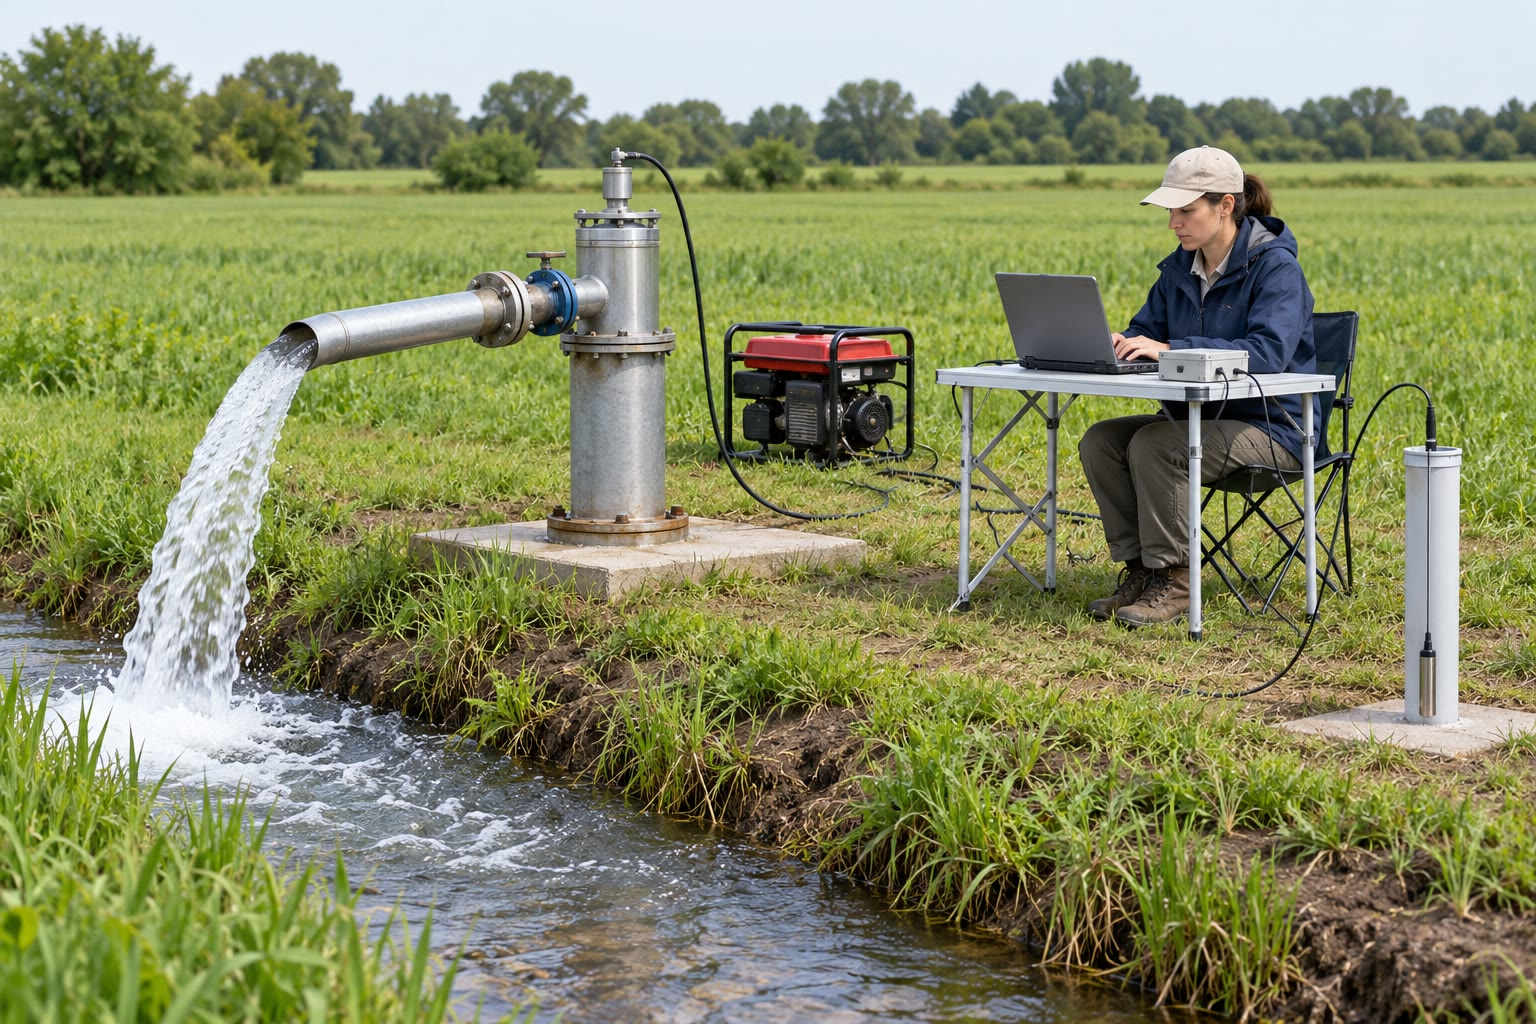
\includegraphics[width=\linewidth]{images/book5/ai/b3-pumping-test.jpg}

{\scriptsize Una prueba de bombeo: la tubería de descarga del pozo bombeado, un
generador y un hidrogeólogo registrando en un ordenador portátil los niveles de un pozo de
observación (Ilustración generada por IA.)}
\end{minipage}
\end{inthefield}
% ledger: heath:theis, heath:jacob, heath:water-levels, usgs:transducers

\section{Transporte de solutos}\label{sec:b3:hydrogeology:transport}

Un soluto disuelto en el agua subterránea es arrastrado por el agua, a la
\omterm{def:b3:hydrogeology:seepage}{velocidad de filtración}, y se dispersa a medida que avanza: el agua de los poros vecinos
se mueve a velocidades y por trayectorias distintas, y el soluto
también se difunde.

\begin{definition}[Dispersión hidrodinámica; dispersividad]\label{def:b3:hydrogeology:ade}
La \emph{dispersión hidrodinámica}\index{dispersión hidrodinámica} es el
esparcimiento de un soluto en el agua subterránea en movimiento debido a las variaciones de la
velocidad del agua de un poro a otro y a la difusión molecular. A lo largo
del flujo se describe mediante un coeficiente de dispersión $D = \alpha_Lv + D^*$,
siendo $v$ la \omterm{def:b3:hydrogeology:seepage}{velocidad de filtración}, $D^*$ la difusividad molecular efectiva y
$\alpha_L$, una longitud, la
\emph{dispersividad}\index{dispersividad} longitudinal del medio.
\end{definition}

\begin{theorem}[Ecuación de advección--dispersión]\label{thm:b3:hydrogeology:ade}
A lo largo de un flujo unidimensional de \omterm{def:b3:hydrogeology:seepage}{velocidad de filtración} constante $v$, la
concentración $C(x, t)$ de un soluto no reactivo cumple
\[
\frac{\partial C}{\partial t} = D\,\frac{\partial^2C}{\partial x^2} -
v\,\frac{\partial C}{\partial x} .
\]
Si la concentración se mantiene en $C_0$ en $x = 0$ desde $t = 0$, en un medio
inicialmente libre de soluto,
\[
\frac{C}{C_0} = \frac12\left[\operatorname{erfc}\frac{x - vt}{2\sqrt{Dt}} +
\mathrm e^{vx/D}\operatorname{erfc}\frac{x + vt}{2\sqrt{Dt}}\right] .
\]
\end{theorem}
\index{ecuación de advección--dispersión}

\begin{proof}
En una rebanada de sección transversal unitaria y longitud $\mathrm dx$, de
porosidad efectiva $n_e$, el soluto almacenado es $n_eC\,\mathrm dx$. Su flujo es
$n_e(vC - D\,\partial C/\partial x)$, arrastrado con el agua y dispersado por
la dispersión, igual que la ley de Fick extiende una sustancia que se difunde. La conservación da
$n_e\partial_tC = -\partial_x[n_e(vC - D\partial_xC)]$, la ecuación. Que
la fórmula la satisface y respeta las condiciones se admite aquí;
el \cref{exo:b3:hydrogeology:12} comprueba su ensanchamiento.
\end{proof}

En el sistema que se mueve con el agua, $\xi = x - vt$, la ecuación es la
ecuación de difusión, y el frente se ensancha como $\sqrt{2Dt} = \sqrt{2\alpha_L
vt} = \sqrt{2\alpha_Lx}$: la anchura del frente crece como la raíz cuadrada
de la distancia recorrida.

\begin{definition}[Factor de retardo]\label{def:b3:hydrogeology:retardation}
Un soluto que se adsorbe sobre los granos, en equilibrio y en proporción
a su concentración, se desplaza más lentamente que el agua. Su
\emph{factor de retardo}\index{factor de retardo (sorción)} es
\[
R = 1 + \frac{\rho_bK_d}{n} ,
\]
$\rho_b$ es la densidad aparente seca del medio, $n$ su porosidad y
$K_d$ el coeficiente de distribución, la masa adsorbida por unidad de masa de
sólido dividida por la concentración en el agua. El soluto se mueve a $v/R$
y se dispersa con $D/R$.
\end{definition}

\begin{omfigure}
\begin{tikzpicture}
\begin{groupplot}[group style={group size=2 by 1, horizontal sep=1.5cm},
  width=0.48\linewidth, height=0.4\linewidth,
  tick label style={font=\scriptsize}, label style={font=\small}, title style={font=\small}]
\nextgroupplot[xlabel={tiempo (días)}, ylabel={$C/C_0$ a \qty{100}{m}},
  xmin=0, xmax=1000, ymin=0, ymax=1.05, title={curvas de llegada},
  legend style={font=\scriptsize, at={(0.97,0.03)}, anchor=south east}]
% computed in figdata/bachelor-3/advection_dispersion.py
\addplot[omDef, thick] table[x=t, y=c1] {figdata/out/bachelor-3-advection_dispersion-btc.dat};
\addlegendentry{$\alpha_L = \qty{1}{m}$}
\addplot[omMeth, thick] table[x=t, y=c3] {figdata/out/bachelor-3-advection_dispersion-btc.dat};
\addlegendentry{$\alpha_L = \qty{3}{m}$}
\addplot[omThm, thick] table[x=t, y=c10] {figdata/out/bachelor-3-advection_dispersion-btc.dat};
\addlegendentry{$\alpha_L = \qty{10}{m}$}
\addplot[black, thick, densely dashed, forget plot] table[x=t, y=cR] {figdata/out/bachelor-3-advection_dispersion-btc.dat};
\node[font=\scriptsize, anchor=west, align=left] at (axis cs:640,0.45) {$\alpha_L = \qty{3}{m}$,\\ $R = 3$};
\addplot[black!40, densely dotted, forget plot] coordinates {(200,0) (200,1.05)};
\nextgroupplot[xlabel={distancia (\unit{m})}, ylabel={$C/C_0$ tras 150 días},
  xmin=0, xmax=160, ymin=0, ymax=1.05, title={perfiles},
  legend style={font=\scriptsize, at={(0.03,0.03)}, anchor=south west}]
\addplot[omDef, thick] table[x=x, y=c1] {figdata/out/bachelor-3-advection_dispersion-profile.dat};
\addlegendentry{$\alpha_L = \qty{1}{m}$}
\addplot[omMeth, thick] table[x=x, y=c3] {figdata/out/bachelor-3-advection_dispersion-profile.dat};
\addlegendentry{$\alpha_L = \qty{3}{m}$}
\addplot[omThm, thick] table[x=x, y=c10] {figdata/out/bachelor-3-advection_dispersion-profile.dat};
\addlegendentry{$\alpha_L = \qty{10}{m}$}
\addplot[black!40, densely dotted, forget plot] coordinates {(75,0) (75,1.05)};
\end{groupplot}
\end{tikzpicture}

\par\smallskip{\small Un soluto inyectado de forma continua en $x = 0$ en un
flujo de \omterm{def:b3:hydrogeology:seepage}{velocidad de filtración} \qty{0.5}{m/d}. A la izquierda, la concentración
a \qty{100}{m} aguas abajo, frente al tiempo: el propio agua llega tras
200 días (línea de puntos); cuanto mayor es la \omterm{def:b3:hydrogeology:ade}{dispersividad}, antes aparecen las primeras
trazas, y más tarde se alcanza la concentración plena. Un soluto adsorbido con $R =
3$ llega tres veces más tarde. A la derecha, la concentración a lo largo del flujo tras
150 días, cuando el agua ha recorrido \qty{75}{m}
(línea de puntos).}\label{fig:b3:hydrogeology:transport}
\end{omfigure}

Las \omterm{def:b3:hydrogeology:ade}{dispersividades} son difíciles de medir y, en la práctica, a menudo se fijan mediante
reglas empíricas. La más antigua toma la \omterm{def:b3:hydrogeology:ade}{dispersividad} longitudinal como una décima parte de
la longitud del penacho. Una recopilación de medidas de campo publicada en
1992 muestra que la \omterm{def:b3:hydrogeology:ade}{dispersividad} crece con la escala del experimento,
que los valores fiables a gran escala son pocos y que, a una escala dada, los
valores se reparten a lo largo de dos o tres órdenes de magnitud.
% ledger: epa:dispersivity

\section{Ejercicios}

\begin{exercise}[$\star$]\label{exo:b3:hydrogeology:1}
Dos piezómetros se sitúan uno junto al otro en un terreno a \qty{120.0}{m} sobre el
datum. El primero tiene la rejilla filtrante a \qty{40}{m} de profundidad y su agua se sitúa
a \qty{12.5}{m} bajo el terreno; el segundo tiene la rejilla filtrante a \qty{80}{m}
de profundidad, su agua a \qty{15.0}{m} bajo el terreno. Calcúlense la altura
de posición, la altura de presión y la \omterm{def:b3:hydrogeology:head}{carga hidráulica} en ambas rejillas. ¿En qué sentido circula el
agua entre ellos, y con qué gradiente vertical?
\end{exercise}

\begin{exercise}[$\star$]\label{exo:b3:hydrogeology:2}
Una columna de arena de \qty{50}{cm} de longitud y \qty{10}{cm} de diámetro, con $K =
\qty{12}{m/d}$ y una porosidad eficaz de 0.35, transporta agua bajo una
diferencia de carga de \qty{30}{cm}. Calcúlense el \omterm{def:b3:hydrogeology:darcy}{caudal específico}, el caudal
en litros por hora y la \omterm{def:b3:hydrogeology:seepage}{velocidad de filtración}.
\end{exercise}

\begin{exercise}[$\star$]\label{exo:b3:hydrogeology:3}
Una caliza tiene $K = \qty{2.5}{m/d}$ para agua a \qty{10}{\celsius}
($\rho = \qty{999.7}{kg/m^3}$, $\mu = \qty{1.306e-3}{Pa.s}$). Calcúlense su
\omterm{def:b3:hydrogeology:darcy}{permeabilidad intrínseca} y su \omterm{def:b3:hydrogeology:darcy}{conductividad hidráulica} para agua a
\qty{20}{\celsius} ($\rho = \qty{998.2}{kg/m^3}$, $\mu =
\qty{1.002e-3}{Pa.s}$).
\end{exercise}
% ledger: nist:water

\begin{exercise}[$\star$]\label{exo:b3:hydrogeology:4}
La caliza confinada de Varden-3 tiene \qty{180}{m} de espesor, con $K =
\qty{2.5}{m/d}$. Calcúlense su \omterm{def:b3:hydrogeology:storage}{transmisividad} y el \omterm{def:b3:hydrogeology:storage}{coeficiente de almacenamiento} que tendría si
solo la expansión del agua, \num{9e-7} por metro de acuífero y por metro de carga, liberara agua.
Compárese con $S = \num{2e-4}$.
\end{exercise}
% ledger: heath:storage

\begin{exercise}[$\star\star$]\label{exo:b3:hydrogeology:5}
Tras un largo período de bombeo a \qty{1500}{m^3/d}, los descensos han
dejado de variar: \qty{2.35}{m} en un pozo de observación a \qty{20}{m} del
pozo de bombeo y \qty{0.82}{m} en uno a \qty{200}{m} de distancia. El acuífero es
confinado y de \qty{40}{m} de espesor. Calcúlense su \omterm{def:b3:hydrogeology:storage}{transmisividad} y su \omterm{def:b3:hydrogeology:darcy}{conductividad
hidráulica}.
\end{exercise}

\begin{exercise}[$\star\star$]\label{exo:b3:hydrogeology:6}
Un pozo bombea \qty{1200}{m^3/d} desde un \omterm{def:b3:hydrogeology:aquifer-types}{acuífero confinado} con $T =
\qty{300}{m^2/d}$ y $S = \num{5e-4}$. Calcúlense $u$, $W(u)$ (a partir de la
serie) y el descenso a \qty{300}{m} de distancia tras 1 día y tras 10 días.
\end{exercise}

\begin{exercise}[$\star\star$]\label{exo:b3:hydrogeology:7}
Para la prueba de Varden-3 ($T = \qty{450}{m^2/d}$, $S = \num{2e-4}$), ¿tras cuántos
minutos puede usarse la recta de Cooper--Jacob en los pozos de observación a \qty{60}{m} y
\qty{500}{m} del pozo de bombeo? ¿Qué indica esto sobre dónde deben situarse los
pozos de observación de una prueba corta?
\end{exercise}

\begin{exercise}[$\star\star$]\label{exo:b3:hydrogeology:8}
Dos pozos separados \qty{400}{m} en la caliza de Varden bombean cada uno
\qty{2160}{m^3/d}. Calcúlese el descenso tras 10 días a mitad de camino entre ambos,
y en el emplazamiento del segundo pozo, debido solo al primero. ¿Por qué el bombeo de cada
pozo le cuesta dinero al otro?
\end{exercise}

\begin{exercise}[$\star\star$]\label{exo:b3:hydrogeology:9}
En la \omterm{def:b3:hydrogeology:flow-net}{red de flujo} bajo la presa, cuéntense los canales de flujo y las caídas de carga.
Con $K = \qty{5}{m/d}$ y $H = \qty{10}{m}$, calcúlese la filtración por
metro de presa y bajo una presa de \qty{300}{m} de longitud.
\end{exercise}

\begin{exercise}[$\star\star\star$]\label{exo:b3:hydrogeology:10}
Modélese una arena limpia como tubos rectos de radio \qty{50}{\micro\metre} con una
porosidad de 0.30. Calcúlense $k$ y $K$ (para agua a \qty{20}{\celsius}, como en el
\cref{exo:b3:hydrogeology:3}),
y compárense con el intervalo típico de la arena limpia. ¿Qué rasgos de una arena real
deja fuera el modelo y en qué sentido desplaza cada uno $K$?
\end{exercise}
% ledger: nist:water, heath:k-chart

\begin{exercise}[$\star\star\star$]\label{exo:b3:hydrogeology:11}
(a)~Muéstrese que el descenso de Cooper--Jacob se anula en $r_0 =
\sqrt{2.25\,Tt/S}$. (b)~Calcúlese $r_0$ tras 30 días de bombeo en la
caliza confinada de Varden, y para la misma roca libre, con $S =
0.2$. (c)~¿Por qué el cono de un \omterm{def:b3:hydrogeology:aquifer-types}{acuífero confinado} puede alcanzar un límite que la
prueba no estaba pensada para detectar?
\end{exercise}
% ledger: heath:jacob, heath:storage

\begin{exercise}[$\star\star\star$]\label{exo:b3:hydrogeology:12}
(a)~Para una distancia de recorrido larga, la curva de llegada en $x$ se aproxima a una
distribución normal en el tiempo, de media $x/v$ y desviación típica $\sigma_t
= \sqrt{2\alpha_Lx}/v$. Demuéstrese a partir del ensanchamiento $\sqrt{2Dt}$ del frente.
(b)~A \qty{100}{m}, con $v = \qty{0.5}{m/d}$, la concentración alcanza
\qty{16}{\percent} tras \num{152.6}~días y \qty{84}{\percent} tras
\num{247.2}~días. Estímese $\alpha_L$. (c)~Un acuífero arenoso tiene $\rho_b =
\qty{1.9}{g/cm^3}$ y $n = 0.30$; un soluto tiene $K_d =
\qty{0.32}{cm^3/g}$. Calcúlese $R$.
\end{exercise}

\section{Problema: prueba de bombeo en Varden-3}

\begin{problem}[{Problema de fin de semana --- cargas, una prueba de bombeo y el recorrido
de un contaminante en la caliza confinada de las colinas de Varden}]
\label{pb:b3:hydrogeology:1}
El pozo ficticio Varden-3 se perfora en (4500, 5000) sobre la cuadrícula de
las colinas de Varden, desde una cota de \qty{363.2}{m}, atravesando la lutita
jurásica hasta la caliza jurásica, cuyo techo queda a
\qty{282.5}{m} y cuya base a \qty{102.5}{m} sobre el nivel del mar; el pozo está abierto
en todo el espesor de la caliza. Antes de la prueba, el agua del pozo se sitúa
a \qty{45.0}{m} por debajo del suelo.

\medskip\noindent\textbf{Parte I --- El acuífero y su flujo natural.}
\begin{enumerate}
\item Calcúlense los espesores de la lutita y de la caliza en el pozo.
\item Calcúlense la \omterm{def:b3:hydrogeology:head}{carga hidráulica} en la caliza y la carga de presión en su techo.
  ¿Por qué la caliza es aquí un \omterm{def:b3:hydrogeology:aquifer-types}{acuífero confinado}?
\item Tres piezómetros abiertos a la caliza se sitúan en P1 (4300, 5250), P2
  (4850, 5150) y P3 (4550, 4650), con cargas de 318.96, 317.34 y
  \qty{317.52}{m}. Si se escribe $h = ax + by + c$, calcúlense $a$ y $b$.
\item Calcúlense el \omterm{def:b3:hydrogeology:head}{gradiente hidráulico} y el acimut hacia el que fluye el
  agua.
\end{enumerate}

\medskip\noindent\textbf{Parte II --- La prueba de bombeo.} El pozo se bombea
a \qty{2160}{m^3/d} durante dos días. En un pozo de observación a \qty{60}{m}
de distancia, los descensos son:
\begin{center}
\begin{tabular}{l*{11}{c}}
\hline
$t$ (\unit{min}) & 1 & 2 & 3 & 5 & 7 & 10 & 15 & 20 & 30 & 45 & 60\\
$s$ (\unit{m}) & 0.18 & 0.36 & 0.48 & 0.64 & 0.77 & 0.88 & 1.04 & 1.15 & 1.30 & 1.45 & 1.56\\
\hline
$t$ (\unit{min}) & 90 & 120 & 180 & 240 & 360 & 480 & 720 & 960 & 1440 & 2160 & 2880\\
$s$ (\unit{m}) & 1.71 & 1.82 & 1.98 & 2.08 & 2.24 & 2.35 & 2.50 & 2.61 & 2.77 & 2.92 & 3.03\\
\hline
\end{tabular}
\end{center}
\begin{enumerate}[resume]
\item Represéntese $s$ frente a $\log_{10}t$. ¿Cuáles de los primeros puntos se apartan de la
  recta, y por qué?
\item A partir del tramo recto, mídase el descenso por ciclo logarítmico.
\item Calcúlese la \omterm{def:b3:hydrogeology:storage}{transmisividad}.
\item Hállese el tiempo $t_0$ en el que la recta corta al descenso nulo.
\item Calcúlese el \omterm{def:b3:hydrogeology:storage}{coeficiente de almacenamiento}.
\item Compruébese que $u \le 0.05$ para los puntos utilizados.
\item Calcúlese la \omterm{def:b3:hydrogeology:darcy}{conductividad hidráulica} de la caliza.
\end{enumerate}

\medskip\noindent\textbf{Parte III --- El cono.} A partir de aquí se toman $T =
\qty{450}{m^2/d}$ y $S = \num{2e-4}$.
\begin{enumerate}[resume]
\item Calcúlese el descenso de Theis en el pozo de observación tras 2 días y
  compárese con el registro.
\item Un pozo de granja a \qty{1}{km} de distancia extrae de la misma caliza. Calcúlese su
  descenso tras 30 días de bombeo.
\item Calcúlese la distancia de Jacob $r_0$ tras 30 días. ¿Qué indica sobre
  los bordes del acuífero y la falla de las colinas de Varden?
\item Calcúlese el volumen bombeado en 30 días. ¿De dónde procede, en un \omterm{def:b3:hydrogeology:aquifer-types}{acuífero confinado},
  ese volumen?
\item ¿Cómo se compararía el descenso en la granja si la caliza fuera
  libre, con $S = 0.18$?
\end{enumerate}

\medskip\noindent\textbf{Parte IV --- Un contaminante.} Una fuga de un contaminante disuelto
llega a la caliza a \qty{200}{m} del pozo. Tómense
una porosidad efectiva de 0.18 y un \omterm{def:b3:hydrogeology:retardation}{factor de retardo} de 2.5.
\begin{enumerate}[resume]
\item Antes del bombeo, calcúlense el \omterm{def:b3:hydrogeology:darcy}{caudal específico} y la \omterm{def:b3:hydrogeology:seepage}{velocidad de filtración}
  del flujo natural de la Parte~I.
\item ¿Cuánto tardaría el agua en recorrer \qty{200}{m}, y el
  contaminante?
\item Con el pozo en bombeo y la fuga aguas arriba de él, el flujo
  se vuelve radial hacia el pozo. Demuéstrese que el agua tarda $t = \pi n_e b
  r^2/Q$ en llegar al pozo desde una distancia $r$, despreciando el flujo
  natural, y calcúlese para el agua y para el contaminante.
\item Con la regla práctica de una \omterm{def:b3:hydrogeology:ade}{dispersividad} igual a una décima parte de la distancia,
  estímese el ensanchamiento $\sqrt{2\alpha_Lx}$ del frente en el pozo. ¿Qué
  significa para la primera llegada?
\item ¿Debe seguir el bombeo? Señálese un argumento a favor y otro en contra.
\item Indíquese la \omterm{def:b3:hydrogeology:storage}{transmisividad} del acuífero de caliza de Varden, en metros cuadrados por día,
  con dos cifras significativas.
\end{enumerate}
\end{problem}
% ledger: heath:jacob, heath:theis, heath:storage, epa:dispersivity, region:name
